\documentclass{report}
\usepackage{tocloft}
\usepackage{geometry}
\usepackage{graphicx}
\usepackage{caption}
\usepackage[T1]{fontenc}
\usepackage[utf8]{inputenc}
\usepackage[polish]{babel}
\usepackage{float}
\usepackage{listings}
\usepackage{xcolor}

\geometry{
    a4paper,
    left=2.5cm,
    right=2.5cm,
    top=2.5cm,
    bottom=2.5cm,
}

\lstset{
    language=Matlab, 
    basicstyle=\footnotesize\ttfamily,
    keywordstyle=\color{blue},
    commentstyle=\color{green},
    stringstyle=\color{red},
    numbers=left,
    numberstyle=\tiny\color{gray},
    stepnumber=1,
    numbersep=5pt,
    backgroundcolor=\color{lightgray},
    frame=single,
    tabsize=2,
    captionpos=b,
    breaklines=true
}


\setcounter{tocdepth}{3}
\setlength{\cftbeforechapskip}{15pt} 
\setlength{\cftbeforesecskip}{8pt} 
\setlength{\cftbeforesubsecskip}{5pt} 
\setlength{\cftbeforesubsubsecskip}{5pt}

\renewcommand\thesection{\arabic{section}.}
\renewcommand\thesubsection{\thesection\arabic{subsection}.}
\renewcommand\thesubsubsection{\thesubsection\arabic{subsubsection}.}
\setcounter{secnumdepth}{3}


\begin{document}


\begin{titlepage}
    \centering
    \vspace*{1cm}
    \begin{figure}
        \centering 
        
\includegraphics[width=0.5\textwidth]{"src/logo.png"}
    \end{figure}
    \Huge
    Zajęcia Projektowe
    \par
    \textbf{Podstawy Robotyki}
    
    \vspace*{1cm}

    \vspace{0.5cm}
    \LARGE \textit{Platforma jeżdżąca automatycznie utrzymująca odległość od ściany}
    
    \vspace{1.5cm}
    
    \textbf{Autorzy:} 
    \par
    Jakub Pająk 
    \par
    Łukasz Grabarski
    \par 
    Krzysztof Grądek
    \par 
    Piotr Legień
    \par
    Bartosz Wuwer
    \vspace*{1.5cm}
    \par AiR Grupa 5TI
    
    \vfill
    
    \Large 30.05.2024
    
\end{titlepage}


\newpage

\tableofcontents

\newpage


\section{\LARGE Wprowadzenie}
\subsection{\Large Cel projektu}
Celem niniejszego projektu jest opracowanie mobilnej platformy robotycznej, zdolnej do automatycznego utrzymywania określonej odległości od ściany. Platforma ta bazować będzie na mikrokontrolerze Arduino oraz laserowych czujnikach odległości typu ToF (ang. Time of Flight). Projekt ma na celu zbadanie i rozwinięcie zaawansowanych algorytmów sterowania i nawigacji, które umożliwią precyzyjne śledzenie ścian w zmiennych warunkach środowiskowych. Dodatkowym celem jest stworzenie wszechstronnego rozwiązania, które można łatwo dostosować do różnych zastosowań, takich jak roboty sprzątające, inspekcyjne czy systemy autonomiczne w logistyce.

\subsection{\Large Założenia wstępne}
Robot zostanie zaprojektowany w oparciu o mikrokontroler Arduino Uno R4, wybrany ze względu na wbudowany moduł Bluetooth LE (LE - Low Energy), co umożliwi zdalne monitorowanie i kontrolę. Silniki zastosowane w projekcie muszą być wyposażone w enkodery, bądź umożliwiać ich dołączenie, co zapewni precyzyjne sterowanie. Czujniki odległości zostaną podłączone do mikrokontrolera za pomocą magistrali I2C. Ze względu na planowaną liczbę czujników (osiem), połączenie ich innymi metodami nie byłoby efektywne.

Zasilanie platformy musi być wystarczające do obsługi co najmniej jednego mikrokontrolera oraz czterech silników. Optymalnym rozwiązaniem będzie zastosowanie czterech ogniw litowo-jonowych połączonych w konfiguracji 2S2P, co zapewni odpowiednią wydajność energetyczną. Dodatkowo, konieczne jest zastosowanie układu zarządzania baterią BMS (ang. Battery Management System), który zabezpieczy ogniwa przed nadmiernym rozładowaniem i przeładowaniem.

Całość konstrukcji zostanie zamknięta w obudowie wykonanej techniką druku 3D. Obudowa będzie podzielona na dwie główne sekcje: dolną, w której zostaną umieszczone silniki oraz ogniwa wraz z układem BMS, oraz górną, zawierającą płytkę stykową, mikrokontroler oraz czujniki. Taka konstrukcja zapewni łatwy dostęp do kluczowych komponentów i umożliwi ich sprawną wymianę w razie potrzeby.

Początkowo plan realizacji projektu zakładał stworzenie aplikacji, która byłaby odpowiedzialna za zdalne sterowanie robotem poprzez moduł BLE (ang. Bluetooth Low Energy). W wyniku późniejszych konsultacji plan uległ zmianie jednak aplikacja zostanie wykorzystana jako wsparcie dla automatycznego trybu robota.

% \subsection{\Large Harmonogram realizacji projektu}
% \subsubsection{\large Okres 1}
% Wykonanie projektu obuydowy robota. Wykonanie bazy aplikacji mobilnej w celu 

\section{\LARGE Realizacja projektu}
Projekt był realizowany etapami, jednak nie został zastosowany szczegółowy harmonogram. 
Przybliżone etapy rozwoju projektu:
\begin{enumerate}
    \item Napisanie aplikacji w wersji dedykowanej systemowi Android w języku Dart,
    \item Realizacja prostego skryptu w Arduino IDE w celu weryfikacji połączenia BLE z mikrokontrolerem,
    \item Wykonanie projektu obudowy robota w 3D oraz przygotowanie do druku,
    \item Wykonanie prostego kodu w celu weryfikacji poprawności podłączenia silników do sterownika,
    \item Podłączenie oraz weryfikacja poprawności działania laserowych czujników odległości,
    \item Montaż silników wewnątrz dolnej komory obudowy,
    \item Montaż ogniw wraz z układem BMS,
    \item Integracja czujników z silnikami oraz implementacja logiki sterowania,
    \item Testy poprawności działania algorytmu sterującego.
\end{enumerate}

\subsection{\Large Panel sterowania w aplikacji}
Podczas analizy możliwych rozwiązań problemu zdalnego sterowania robotem wybór padł na wykonanie aplikacji mobilnej oraz przesyłanie odpowiednich komend za pomocą protokołu BLE. Protokół BLE jest pewnym szczególnym przypadkiem ogólnego protokołu Bluetooth, jest on szczególnie często spotykany w przypadku mniej zaawansowanych mikrokontrolerów takich jak Arduino Uno R4. Dzięki odpowiedniej architekturze, protokól ten pozwala na bardziej efektywne zarządzanie pobieraną energią jednocześnie zachowując niezbędne funkcjonalności. 

Przez wzgląd na wcześniej nabyte umijętności tworzenia aplikacji za pomocą języka Dart przez jednego z członków sekcji, prace nad projektem rozpoczęto od implementacji podstawowej wersji aplikacji realizującej proste przesyłanie informacji w postaci całkowitoliczbowej w celu późniejszej interpretacji otrzymanych danych w środowisku Arduino. 

Przez wzgląd na tematykę projektu implementacja aplikacji nie zostanie w poniższym raporcie szczegółowo omówiona. Zostanie przedstawiony podstawowy interfejs graficzny oraz zasada działania kluczowych funkcji, takich jak połączenie lub realizacja przesyłu danych. Autor uważa, iż pewne wyszczególnienie części metod oraz zastosowanych bibliotek może pomóc niektórym osobom w prostrzym znalezieniu informacji na temat poprawnie działającego połączenia z mikrokontrolerem Arduino poprzez Bluetooth.

\subsubsection{\large Interfejs użytkownika aplikacji }
% --------------------------------------------------------
% Autor: Jakub Pajak
% TODO: Opisać Interfejs użytkownika oraz co robią poszczególne funkcje, jak działa aplikacja na poziomie ideowym
%
% Status: 
% --------------------------------------------------------

\subsection{\Large Implementacja połączenia Bluetooth}
% --------------------------------------------------------
% Autor: Jakub Pajak
%
% TODO: Opisać zasadę działania połączenia Bluetooth poprzez paczkę flutter_blue
%
% Status: 
% --------------------------------------------------------

\subsection{\Large Implementacja przesyłania danych}
% --------------------------------------------------------
% Autor: Jakub Pajak
%
% TODO: Opisać sposób przekazywania infomracji o przyciśniętym przycisku w postaci całkowitoliczbowej
%
% Status: 
% --------------------------------------------------------


\subsection{\Large Implementacja prostego skryptu w odczytującego dane z kanału BLE }
Fragment prezentowanego kodu rozpoczyna się od zadeklarowania zmiennych globalnych opisujących charakterystyki połączenia Bluetooth. Pierwsza charakterystyka określa identyfikator typu GUID serwisu, następna określa na jaki identyfikator przesyłane są zdarzenia typu "request". Ostatnia wartość definiuje indentyfikator na jaki są przesyłane zdarzenia typu 'response". 
W przypadku aktualnej wersji aplikacji istotna jest tylko wartość identyfikująca serwis oraz zdarzenia typu request, ponieważ mikrokontroler nie zwraca żadnej informacji do aplikacji. W razie dalszego rozwoju projektu zostanie zaimplementowanie wyświetlanie diagnostyki robota, stanu naładowania baterii oraz stanu pracy silników. 

Funkcja \texttt{t5Callback()} ma za zadanie pobierać wartość która aktualnie została przesłana do kanału Bluetooth z poziomu aplikacji. Argumenty wejściowe funkcji to urządzenie z którym Arduino nawiązało połączenie, drugi argument to wcześniej wspomniany identyfikator zdarzenia "request".

Następnie wartość jest odczytywana z kanału za pomocą funkcji \texttt{readValue()}. Funkcja ta jest częścią biblioteki \texttt{ArduinoBLE.h}.

W funkcji \texttt{setup()} następuje inicjalizacja odpowiednich charakterystyk oraz za pomocą funkcji \newline \texttt{setEventHandler()} zostaje określona sytuacja w której nastąpi wywołanie funkcji \texttt{t5Callback} oraz odczytanie danych z kanału. 

\begin{figure}[H]
    \centering
    \includegraphics*[width=1.0\textwidth]{"src/code_snaps/bt_con_arduino.png"}
    \caption{Fragment kodu źródłowego przedstawiający implementację konfiguracji kanału Bluetooth na Arduino}
    \label{fig:bt_con_arduino}
\end{figure}


\newpage
\subsection{\Large Proces wykonywania projektu obudowy robota}
% --------------------------------------------------------
% Autor: Łukasz Grabarski
%
% TODO: Opisać proces oraz sposób wykonania projektu obudowy w 3D
%
% Status: 100%
% --------------------------------------------------------

Proces projektowania obudowy dla platformy jeżdżącej stanowił wieloetapowe zadanie, które wymagało dokładnego zaplanowania i licznych poprawek. Pierwsza faza obejmowała stworzenie prototypu, który miał na celu optymalne rozmieszczenie komponentów oraz weryfikację ich poprawnego działania. 
Ten etap pozwalał zidentyfikować ewentualne problemy konstrukcyjne i funkcjonalne na wczesnym etapie prac.

\begin{figure}[H]
    \centering
    \includegraphics*[width=0.4\textwidth]{"src/Robot_pics/Build_1.jpg"}
    \caption{Prototypowa konstrukcja mająca na celu sprawdzenie poprawności działania komponentów.}
    \label{fig:bt_con_arduino}
\end{figure}

Kolejnym krokiem było opracowanie specjalnej obudowy, zdolnej pomieścić wszystkie wymagane elementy, przy jednoczesnym zachowaniu odpowiedniej geometrii kół szwedzkich (zwanych również kołami Mecanum). 
Aby robot działał zgodnie z założeniami, koła musiały być rozmieszczone w orientacji X Y równych odstępach od siebie, a ich rolki powinny być skierowane do środka. Konieczne jest aby z rzutu górnego posiadał przedłużenie osi kół w kształcie znaku X. 


\begin{figure}[H]
    \centering
    \includegraphics*[width=0.5\textwidth]{"src/Robot_pics/Mecanum_lines.png"}
    \caption{Plan rozmieszczenia kół szwedzkich. Kluczowe jest zachowanie kół w równych odstępach od siebie oraz utworzenie znaku X.}
    \label{fig:bt_con_arduino}
\end{figure}


\begin{figure}[H]
    \centering
    \includegraphics*[width=1.0\textwidth]{"src/Robot_pics/blender.png"}
    \caption{Pierwsza wersja projektu zamodelowana w programie Blender 4.1.}
    \label{fig:bt_con_arduino}
\end{figure}

Jednakże podczas pierwszego etapu projektu nastąpiły problemy logiczne i konstrukcyjne. Pierwotnie używany darmowy program Blender 4.1 okazał się niewystarczający ze względu na niezgodność formatów eksportu z wymaganiami dostępnej drukarki 3D. 
W związku z tym, konieczne było przejście na bardziej zaawansowane narzędzie, jakim jest AutoDesk Fusion. To oprogramowanie pozwoliło na dokładniejsze zaprojektowanie modelu, uwzględniając specyfikację drukarki, która posiadała obszar roboczy o wymiarach 25 cm x 25 cm. 
Z tego powodu, model musiał zostać zaprojektowany od nowa, z uwzględnieniem ograniczeń.

\begin{figure}[H]
    \centering
    \includegraphics*[width=1.0\textwidth]{"src/Robot_pics/Fusion 1.png"}
    \caption{Wizualizacja gotowego modelu w programie AutoDesk Fusion.}
    \label{fig:bt_con_arduino}
\end{figure}

\newpage

Gotowy produkt składa się z dwóch pięter, z których każde pełni inną funkcje. 
Pierwsze piętro to "piętro maszynowe", gdzie umieszczone zostały moduły napędowe, takie jak silniki kątowe z przekładnia oraz ogniwa zasilające w ilości dwóch wraz ze sterownikiem BMS. 
Wszystkie istotne kable zostały przeprowadzone przez specjalnie przygotowany otwór do drugiego piętra.

\begin{figure}[htbp]
    \centering
    \begin{minipage}[b]{0.45\textwidth}
        \centering
        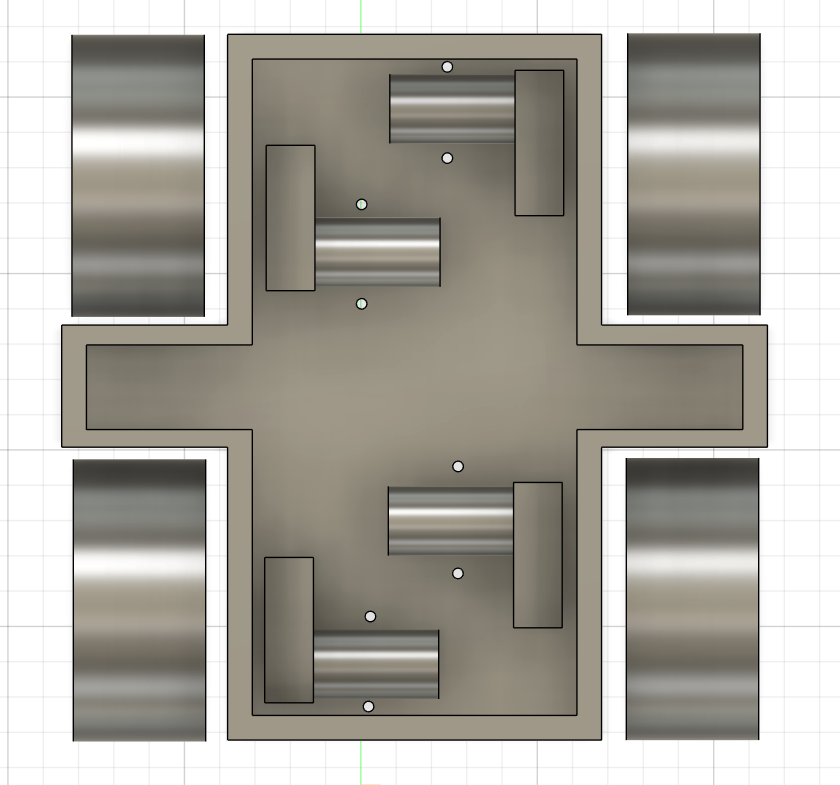
\includegraphics[width=\textwidth]{"src/Robot_pics/Dol.png"}
        \caption{Widok rzutu górnego na pierwsze piętro modelu. Znajdują się w nim silniki kątowe z przekładnią oraz miejsce na ogniwa zasilające wraz z BMS.}
        \label{fig:zdjecie1}
    \end{minipage}
    \hfill
    \begin{minipage}[b]{0.45\textwidth}
        \centering
        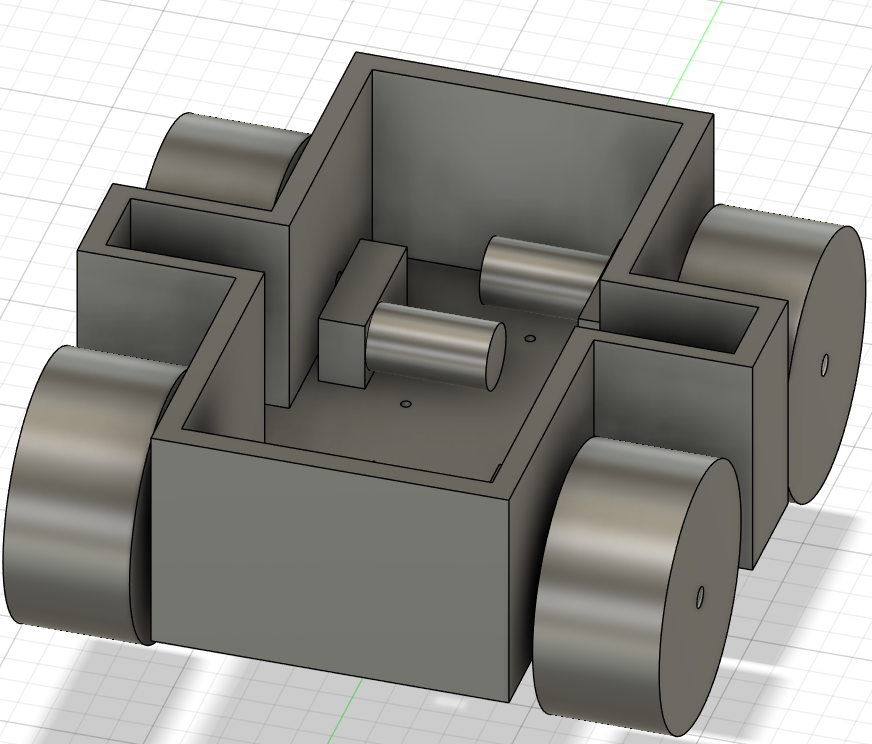
\includegraphics[width=\textwidth]{"src/Robot_pics/Dol 1.png"}
        \caption{Widok rzutu bocznego na pierwsze piętro modelu.}
        \label{fig:zdjecie2}
    \end{minipage}
\end{figure}

Drugie piętro to "mózg operacyjny" całego projektu. Zawiera ono kluczowe połączenia elektroniczne, w tym dwa mikrokontrolery Arduino UNO 4 i 3 w konfiguracji Master-Slave, oraz osiem czujników laserowych umieszczonych w przygotowanych otworach na ścianach bocznych. 
Takie rozmieszczenie i organizacja komponentów pozwalają na efektywne zarządzanie funkcjami robota.

\begin{figure}[htbp]
    \centering
    \begin{minipage}[b]{0.45\textwidth}
        \centering
        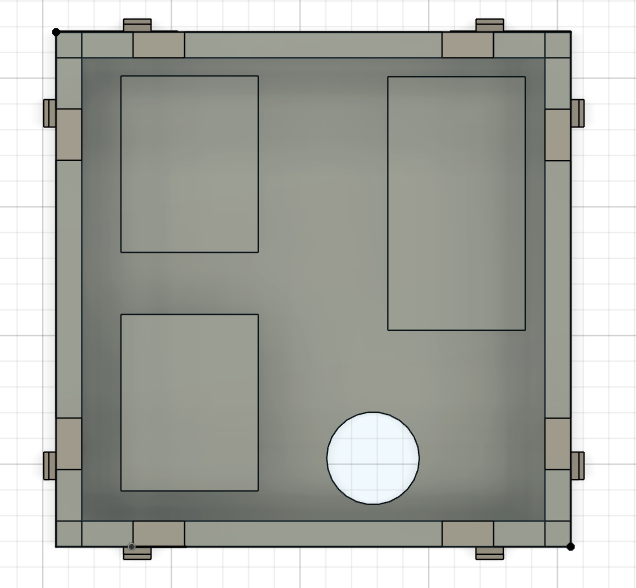
\includegraphics[width=\textwidth]{"src/Robot_pics/Gora.png"}
        \caption{Widok rzutu górnego na drugie piętro modelu. Znajdują się w nim dwa mikronotrolery Arduino UNO oraz płytka stykowa.}
        \label{fig:zdjecie1}
    \end{minipage}
    \hfill
    \begin{minipage}[b]{0.45\textwidth}
        \centering
        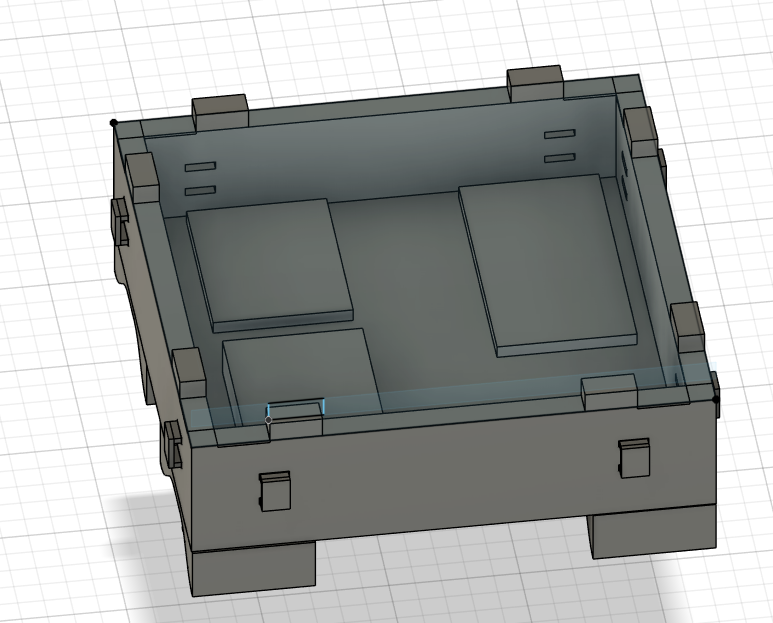
\includegraphics[width=\textwidth]{"src/Robot_pics/Gora 1.png"}
        \caption{Widok rzutu bocznego na drugie piętro modelu.}
        \label{fig:zdjecie2}
    \end{minipage}
\end{figure}

\begin{figure}[H]
    \centering
    \includegraphics*[width=1.0\textwidth]{"src/Robot_pics/Fusion 3.png"}
    \caption{Widok rzutu bocznego na specjalnie przygotowane miejsca do wsunięcia czujników laserowych.}
    \label{fig:bt_con_arduino}
\end{figure}

\begin{figure}[H]
    \centering
    \includegraphics*[width=1.0\textwidth]{"src/Robot_pics/Fusion 2.png"}
    \caption{Gotowy model przesłany do wydruku. Został pozbawiony elementów stylistycznych takich jak koła, silniki kątowe, mikrokontrolerów Arduino UNO oraz czujników laserowych.} 
    \label{fig:bt_con_arduino}
\end{figure}

\newpage

Gotowy model zawiera się w wymiarach 20 cm x 20 cm x 15 cm oraz wykonuje wszystkie zadane ruchy zdolne do wykonania tylko przy pomocy
kół szwedzkich. Pojazd wykonuje jazdę w kierunku w przód i w tył oraz w lewo i w prawo jak i obrót w miejscu.

\begin{figure}[H]
    \centering
    \includegraphics*[width=0.5\textwidth]{"src/Robot_pics/Finished.png"}
    \caption{Gotowy model po złożeniu wszystkich elementów w całość.}
    \label{fig:bt_con_arduino}
\end{figure}



\subsection{\Large Implementacja prostego kodu weryfikującego prawidłowe podłączenie silników}

% --------------------------------------------------------
% Autor: Krzysztof Grądek
%
% TODO: Opisać kod oraz sposób podłączenia silników do sterownika + krótki opis sterownika
%
% Status: 100%
% --------------------------------------------------------

Do połączenia silników z Arduino wykorzystano nakładkę Iduino ST1138. Umożliwia ona sterowanie czterema silnikami prądu stałego, o poborze prądu do 600 mA i napięciu zasilania do 36 V. Nakładka jest zasilana dwoma ogniwami 18650.

Weryfikacja połączenia silników została wykonana przy użyciu skryptu zamieszczonego poniżej. Na początku skryptu dodane są biblioteki Wire i AFMotor. Biblioteka Wire jest wykorzystywana do połączenia obu modułów Arduino w konfiguracji master-slave, natomiast biblioteka AFMotor służy do sterowania silnikami z nakładki Iduino.

W następnych liniach zdefiniowane są: adres urządzenia slave oraz globalna wartość bezpiecznego dystansu, który jest potrzebny, aby w przypadku wystającego gzymsu, który mógłby ominąć czujniki, pojazd nie zahaczył o niego.

Dalsza część kodu zawiera wykorzystanie biblioteki AFMotor i przypisanie konkretnych silników do zmiennych.

W ostatniej części, czyli setup, znajduje się połączenie przez bibliotekę Wire, rozpoczęcie komunikacji z prędkością 9600 bitów na sekundę (Serial.begin(9600)) oraz ustawienie prędkości wszystkich silników.

Do weryfikacji działania silników można zakomentować pozostałe ustawienia setSpeed, tak aby pozostało tylko jedno i sprawdzić, który silnik jest uruchomiony.
\begin{figure}[H]
    \centering
    \includegraphics*[width=1.0\textwidth]{"src/code_snaps/eng_ste_arduino.png"}
    \caption{Framgent kodu źródłowego przedstawiający weryfikacje prawidłowego połączenia silników}
    \label{fig:eng_ste_arduino}
\end{figure}

\subsection{\Large Podłączenie oraz weryfikacja poprawności działania czujników laserowych}

% --------------------------------------------------------
% Autor: Jakub Pająk
%
% TODO: Opisać sposób podłączenia czujników oraz kod weryfikujący podłączenie
%
% Status: 80% done
% --------------------------------------------------------
We wczesnej fazie planowania zakładano wykorzystanie ultradźwiękowych czujników odległości. Pomysł ten okazał się nietrafiony ze względu na sposób przekazywania danych przez te czujniki. Każdy czujnik posiada dwa wyprowadzenia, co przy użyciu ośmiu czujników wymagałoby wykorzystania co najmniej 16 pinów Arduino.

Następnie analiza skupiła się na wykorzystaniu magistrali I2C, która umożliwia podłączenie dużej liczby czujników za pomocą niewielkiej liczby pinów. Kluczowym warunkiem jest poprawna komunikacja między czujnikiem a mikrokontrolerem.

Laserowe czujniki odległości VL530L0X okazały się trafnym wyborem ze względu na ich korzystny stosunek jakości do ceny. Pomiary odległości są wystarczająco dokładne, a biorąc pod uwagę charakter obiektu wykrywanego, wysoka precyzja nie jest wymagana.

Czujniki zostały podłączone zgodnie z przeznaczeniem poprzez magistralę I2C. Kluczową rolę w podłączaniu wielu identycznych czujników odegrało użycie dodatkowego pinu XSHUT oraz odpowiedniej sekwencji kodu, aby pomyślnie zmienić adres czujnika na magistrali I2C. 

Pierwszym krokiem jest ustawienie odpowiedniego pinu GPIO (ang. General Purpose Input/Output) Arduino, podłączonego do pinu XSHUT czujnika, w trybie OUTPUT. Następnie należy skorzystać z funkcji \texttt{setAddress()}, aby ustawić odpowiedni adres dla wybranego czujnika. Kolejnym krokiem jest przełączenie stanu pinu Arduino na INPUT oraz odczekanie 10 milisekund.

Wykonanie powyższej sekwencji gwarantuje poprawną zmianę adresu czujnika na magistrali I2C. Użycie samej funkcji \texttt{setAddress()} bez zastosowania pinu XSHUT nie zmieni adresu czujnika.

\begin{figure}[H]
    \centering
    \includegraphics*[width=0.5\textwidth]{"src/code_snaps/sensor_init.png"}
    \caption{Fragment kodu źródłowego przedstawiający sekwencję konieczną do zmiany adresu czujnika}
    \label{fig:sensor_init}
\end{figure}


\subsection{\Large Montaż silników wewnątrz dolnej komory obudowy}

% --------------------------------------------------------
% Autor: Piotr Legień && Krzysztof Grądek
%
% TODO: Opisać sposób montażu silników oraz usztywnienia wału silnika + montaż kół
%
% Status: 
% --------------------------------------------------------

\subsection{\Large Montaż ogniw wraz z układem BMS oraz podłączenie czujników}

% --------------------------------------------------------
% Autor: Bartosz Wuwer && Piotr Legień
%
% TODO: Opisać sposób połączenia ogniw oraz układ BMS (po co jest etc.)
%
% Status: 
% --------------------------------------------------------

\newpage
\subsection{\Large Integracja czujników z silnikami oraz implementacja logiki sterowania}

% --------------------------------------------------------
% Autor: Jakub Pająk && Łukasz Grabarski
%
% TODO: Opisać kod implementujący integrację czujników z silnikami
%
% Status: Łukasz 50% (jeszcze coś dopiszę)
% --------------------------------------------------------

\subsubsection{\Large Slave}

Mikrokontroler Arduino UNO 3 skonfigurowany do pracy typu Slave odbiera paczkę danych przez zmienną "rd" wysyłane przez Master.

\begin{figure}[H]
    \centering
    \includegraphics*[width=0.4\textwidth]{"src/code_snaps/Comunication_slave.png"}
    \caption{Fragment kodu źródłowego przedstawiający odbiór komunikatów przesyłanych przez mikrokontroler Master.}
    \label{fig:sensor_init}
\end{figure}

Zgodnie z odbieranym komunikatami o zmianie kierunku indeksowanymi od 0 do 3, program wywołuje odpowiednie funkcje. 

\begin{figure}[H]
    \centering
    \includegraphics*[width=0.4\textwidth]{"src/code_snaps/movement_implementation.png"}
    \caption{Fragment kodu źródłowego przedstawiający implementację ruchu pojazdu w odpowiednich kierunkach.}
    \label{fig:sensor_init}
\end{figure}

\newpage

Funkcje określające kierunek jazdy zostały skonstruowane wedle logiki i geometrii działania kół szwedzkich.

\begin{figure}[H]
    \centering
    \includegraphics*[width=0.7\textwidth]{"src/Robot_pics/Movement.png"}
    \caption{Wizualizacja zależności kierunku jazdy od obrotu kół szwedzkich.}
    \label{fig:sensor_init}
\end{figure}

\subsection{\Large Testy poprawności działania algorytmu sterującego}

% --------------------------------------------------------
% Autor: Wszyscy
%
% TODO: Opisać proces testowania oraz rezultaty algorytmu testującego
%
% Status: 
% --------------------------------------------------------

\section{\LARGE Napotkane problemy}
\subsection{\Large Połączenie aplikacji z Arduino}
% --------------------------------------------------------
% Autor: Jakub Pająk
%
% TODO: Opisać problemy napotkane podczas tworzenia aplikacji 
%
% Status: 
% --------------------------------------------------------

\subsection{\Large Podłączenie laserowych czujników odległości}
% --------------------------------------------------------
% Autor: Jakub Pająk
%
% TODO: Opisać problemy podczas podłączenia czujników laserowych
%
% Status: 
% --------------------------------------------------------


\subsection{\Large Montaż silników oraz kół}
% --------------------------------------------------------
% Autor: Wszyscy
%
% TODO: Opisać problemy podczas montażu
%
% Status: 
% --------------------------------------------------------


\section{\LARGE Podsumowanie}
% --------------------------------------------------------
% Autor: Wszyscy
%
% TODO: Napisać zgrabne podsumowanie projektu, czego się nauczyliśmy oraz sensowne wnioski do popełnionych błędów.
%
% Status: 
% --------------------------------------------------------
\end{document}